\documentclass[tikz,border=10pt]{standalone}
\usepackage{amsmath}
\begin{document}
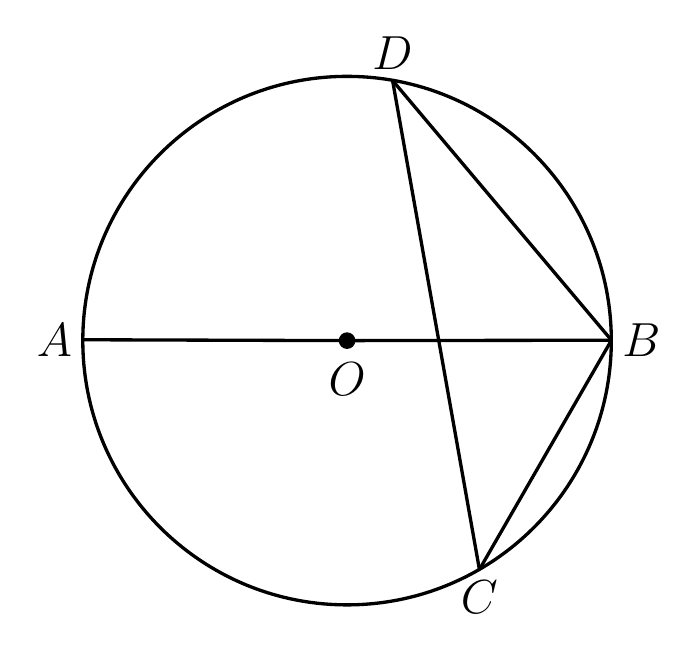
\begin{tikzpicture}[line width=1.2pt, line join=round]
\coordinate (A) at (-3.382,-0.181);
\coordinate (B) at (3.331,-0.187);
\coordinate (C) at (1.654,-3.099);
\coordinate (D) at (0.551,3.112);
\coordinate (O) at (-0.027,-0.192);









\draw (O) circle[radius=3.356];


\draw (A) -- (O) -- (B);
\draw (B) -- (D);
\draw (B) -- (C);
\draw (C) -- (D);


\fill (O) circle (3.000pt);


\node[left] at (A) {\fontsize{18}{21.6}\selectfont $A$};
\node[right] at (B) {\fontsize{18}{21.6}\selectfont $B$};
\node[below] at (C) {\fontsize{18}{21.6}\selectfont $C$};
\node[above] at (D) {\fontsize{18}{21.6}\selectfont $D$};
\node[below=4pt] at (O) {\fontsize{18}{21.6}\selectfont $O$};
\end{tikzpicture}
\end{document}